\begin{frame}
\frametitle{Overview}
    \begin{itemize}
        \item Background
        \item \emph{\color{UOYellow}Methodology}
        \item Results
        \item Future Work
    \end{itemize}
\end{frame}

\begin{frame}
\frametitle{Methodology}
    \begin{itemize}
        \item Generative based machine learning models are a promising avenue
            for time-series upscaling.
        \item Attention based networks are shown to be highly parallelizable and
            able to "remember" features through time-series data. 
        \item Convolutional Neural Networks (CNNs) are computationally efficient and
            have proven effective in working with images.
        \item Model uses CNNs, skip layers, and self-attention to generate
            time-series upscalling.
    \end{itemize}
\end{frame}

\begin{frame}
    \frametitle{Model}
    \center%\documentclass[tikz]{standalone}
%\usepackage{tikz}

%\tikzset{
%    ->, 
%    level distance = 12em,
%    minimum size=2em,
%    %edge from parent/.style={draw,thick},
%    level 1/.style={sibling distance=6em},
%    level 2/.style={sibling distance=3em},
%    thick/.style = {line width=1.5pt},
%    extra thick/.style = {line width=3.5pt},
%    red node/.style={shape=circle,draw=red,fill=red!40,thick,inner sep=1.2},
%    blue node/.style={shape=circle,draw=blue,fill=blue!40,thick,inner sep=1.2}
%}
%
%\tikzstyle{round}=[thick,draw=black,circle]

%\begin{document}

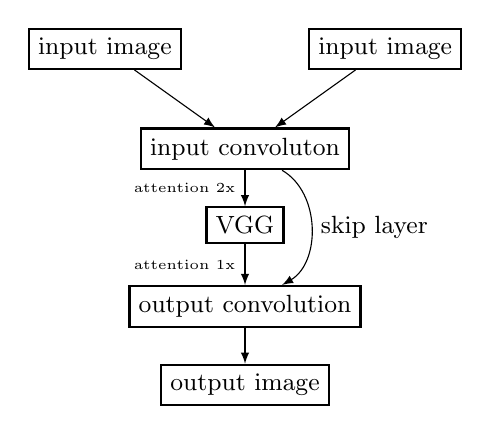
\begin{tikzpicture}[auto,node distance=8mm,>=latex,font=\small]
    \tikzstyle{rec}=[thick,draw=black,rectangle]
    \node[rec, left=8mm] (img1) {input image};
    \node[rec, right=8mm] (img2) {input image};
    \node[rec, below=10mm] (input) {input convoluton};
    \node[rec, below=20mm] (VGG) {VGG};
    \node[rec, below=30mm] (output) {output convolution};
    \node[rec, below=40mm] (outimg) {output image};

    \draw[->] (img1) [] to node {} node [swap] {} (input);
    \draw[->] (img2) [] to node {} node [swap] {} (input);
    \draw[->] (input) [] to node {} node [swap] {\tiny{attention 2x}} (VGG);
    \draw[->] (VGG) [] to node {} node [swap] {\tiny{attention 1x}} (output);
    \draw[->] (output) [] to node {} node [swap] {} (outimg);

    \draw[->] (input) [out=330, in=30] to node {skip layer} node [swap] {} (output);
    %\draw[->] (img1) [out=270,in=145] to node {} node [swap] {} (output);
    %\draw[->] (img2) [out=270,in=35] to node {} node [swap] {} (output);


\end{tikzpicture}

%\end{document}

\end{frame}

